\section{Experiments}\label{sec:experiments}

The experiments ask four questions. How detectable are canaries, and can detectability
be closed by design (Theorem~\ref{thm:detect})? Does an audit with semantic twins
separate memorising from unlearned models on a real language model
(Proposition~\ref{prop:semantic})? Under partial unlearning, does the trained form
disappear before the fact, and does auditing paraphrases change verdicts? How do
membership-inference audits behave on the same runs? Every number below is produced by
a script under \texttt{extension/experiments/}, stored under \texttt{extension/results/},
and turned into the tables of this paper by \texttt{extension/manuscript/make\_tables.py}.
A test suite of eleven tests checks the generators and the exact null without model
weights.

\subsection{Setup}\label{sec:exp-setup}

\paragraph{Data.} The organic records are fictitious biographies drawn from six sentence
templates (birthplace and profession; study city; publication city; years in a city
before a profession; a city guild prize; a workshop near a city) over fictitious first
and last names, cities and professions. These are the keep and forget biographies of the
VOUCH experiments. Each run uses $2{,}000$ keep records, $200$ organic forget records and
a cohort of $m=384$ semantic twin pairs over five attributes (birthplace, profession,
instrument, pet, colour). In-twins are trained in the literal form and one
question--answer form and are repeated $1$, $2$, $4$ or $8$ times by stratum. Belief
scores use four paraphrased questions per attribute, none of which is trained.

\paragraph{Models and training.} The main model is Pythia-410M and the second size is
Pythia-1B \citep{biderman2023pythia}; GPT-2 is used for a pilot and for detector
features. A LoRA adapter \citep{hu2022lora} of rank $16$ on all linear layers is
fine-tuned for $600$ steps (batch $8$, learning rate $2\cdot10^{-4}$, blocks of $96$
tokens). Gradient ascent (GA) and NPO \citep{zhang2024npo} act on a copy of the
fine-tuned adapter with batch $4$ and learning rate $10^{-4}$; NPO uses a retain term on
the keep data and the fine-tuned adapter as its reference. Retraining is a fresh adapter
trained on the keep data only, which satisfies the exact null; no unlearning is the
positive control. All runs were done on single NVIDIA T4 GPUs.

\paragraph{Audit.} Verdicts use the VOUCH engine at $\alpha=0.05$ with a reveal order
drawn from local entropy for the reported runs and from committed seeds for the offline
re-analyses. We report the realised advantage $\hat\Delta$ of the literal score and of
the calibrated belief score (``paraphrase''). Recall that REVOKED rejects the exact null,
some dependence on the coins, at any $\eps$, while ISSUED certifies $|\Delta|<\eps$.

\subsection{Canary detectability}\label{sec:exp-detect}

Theorem~\ref{thm:detect} bounds the gap between canary and organic advantage by twice
the distinguishing advantage $\gamma$. We train two detectors to tell $400$ canary
in-twins from $400$ organic records, both scored out of fold over five folds: a logistic
regression on GPT-2 token-loss features (mean, maximum, median and spread of the token
losses, and length), a trained version of the zero-knowledge perplexity filter of the original study, and a logistic
regression on character $2$--$4$-grams, which requires labelled canaries. A detector's
advantage $\max_\tau|\mathrm{TPR}-\mathrm{FPR}|$ is a lower bound on $\gamma$. For
reference, a detector whose scores are independent of the label exceeds $0.095$ in
$5\%$ and $0.115$ in $1\%$ of $4{,}000$ simulations at this sample size.

\begin{table}[t]
\centering\small
\caption{Detecting canaries among organic records ($400$ canaries, $400$ organic records,
five-fold out-of-fold scores). A detector's advantage is a lower bound on the
distinguishing advantage $\gamma$ of Theorem~\ref{thm:detect}. The null reference for
the advantage is $0.095$ (95th percentile) and $0.115$ (99th).}
\label{tab:detect}
\begin{tabular}{lccccc}
\toprule
 & \multicolumn{2}{c}{Perplexity features} & \multicolumn{2}{c}{Character $n$-grams} & \\
\cmidrule(lr){2-3}\cmidrule(lr){4-5}
Canary design & AUC & advantage & AUC & advantage & $\gamma\ge$ \\
\midrule
VOUCH random-string QA & 0.998 & 0.973 & 1.000 & 1.000 & 1.000 \\
semantic twin, literal & 0.998 & 0.978 & 1.000 & 1.000 & 1.000 \\
semantic twin, question--answer & 0.892 & 0.605 & 1.000 & 1.000 & 1.000 \\
organic-matched twin & 0.521 & 0.052 & 0.442 & 0.102 & 0.102 \\
\bottomrule
\end{tabular}

\end{table}

Table~\ref{tab:detect} compares four designs. VOUCH's random-string records and both forms
of naive semantic twins are detected with advantage one by the $n$-gram classifier, and
the first two also by the zero-knowledge perplexity filter. Random strings, a middle
initial in every canary name and attributes that never occur in organic data give the
cohort away. For these designs Corollary~\ref{cor:ladder} says nothing about organic
records. Organic-matched twins (Section~\ref{sec:matched}) bring both detectors to chance:
the perplexity detector's advantage, $0.052$, is below the 95th percentile of the null
reference, and the $n$-gram detector's, $0.102$, lies between the 95th and the 99th; its
AUC is below one half, so the classifier does not separate the classes in the direction
it was trained for, and the advantage comes from the absolute value in its definition.
These are lower bounds on $\gamma$ against two detector families, not a proof that no
detector exists, which is the conditional nature of Theorem~\ref{thm:detect}. The
original study found that even an entropy-diluted template that defeats the perplexity
filter is still recovered by a trained $n$-gram classifier; matching the organic
generator removes that signature too.

\subsection{Auditing with semantic twins}\label{sec:exp-semantic}

Table~\ref{tab:semantic} audits Pythia-410M when the forget set contains every form the
in-twins were trained in.

\begin{table}[t]
\centering\small
\caption{Semantic-twin audit on Pythia-410M, full forget set ($m=384$, three seeds).
Realised advantages per seed and the two-sided verdict over all scores (I issued, R
revoked, U undetermined).}
\label{tab:semantic}
\begin{tabular}{lllcc}
\toprule
Subject & literal $\hat\Delta$ & paraphrase $\hat\Delta$ & $\eps=0.2$ & $\eps=0.1$ \\
\midrule
no unlearning & $+0.29$, $+0.32$, $+0.46$ & $+0.20$, $+0.27$, $+0.26$ & R R R & R R R \\
GA (100 steps) & $+0.03$, $+0.07$, $-0.05$ & $+0.05$, $+0.05$, $-0.07$ & I I I & I I I \\
NPO (250 steps) & $+0.03$, $-0.09$, $-0.04$ & $+0.07$, $-0.07$, $-0.03$ & I I I & I I I \\
retrain & $-0.03$, $-0.05$, $+0.03$ & $+0.01$, $+0.11$, $+0.08$ & I I I & I U I \\
\bottomrule
\end{tabular}

\end{table}

Paraphrased questions that were never trained carry about two thirds of the literal
advantage, and the audit separates the positive from the negative control in every
seed. A pilot with GPT-2 (128 pairs, 400 training steps) did not: its positive control
reached advantages of $+0.25$ (literal) and $+0.17$ (paraphrase) and was not revoked.
Semantic twins need a model that generalises a stated fact to its paraphrases, which
the smaller model barely does. With the full forget set, GA and NPO remove both
advantages and nothing distinguishes the two scores.

\subsection{Partial unlearning}\label{sec:exp-squeeze}

The case a literal audit cannot see is unlearning that removes the trained surface form
but not the fact. To provoke it we restrict the forget set to the literal statements, so
the question--answer form stays out of it, and sweep the strength of unlearning: GA for
$5$ to $25$ steps and NPO for $10$ to $75$ steps, with eight seeds per model; three of
the Pythia-410M seeds also run GA for $50$ and $100$ steps and NPO for $250$. The
\emph{retention} of a score is its advantage after unlearning divided by the same seed's
advantage before unlearning.

\begin{figure}[t]
\centering
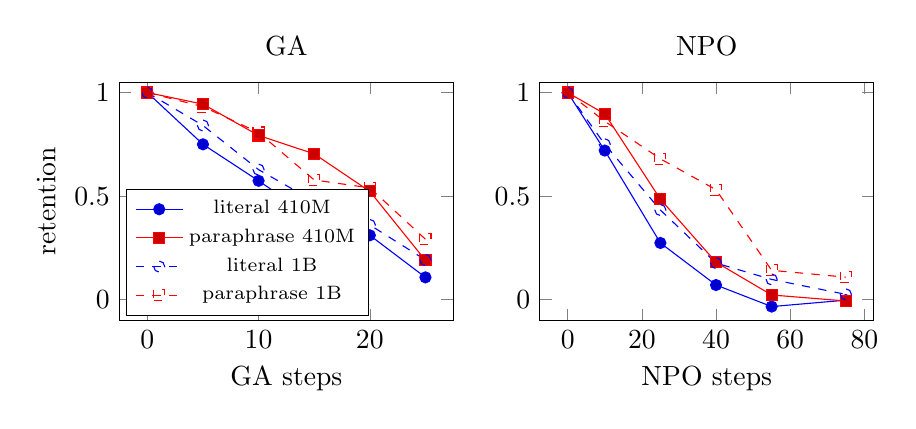
\begin{tikzpicture}
\begin{axis}[name=ga, width=0.48\textwidth, height=0.38\textwidth,
  xlabel={GA steps}, ylabel={retention}, ymin=-0.1, ymax=1.05, title={GA},
  legend style={font=\scriptsize, at={(0.02,0.02)}, anchor=south west}]
\addplot+[mark=*, blue] coordinates {(0,1.000) (5,0.750) (10,0.574) (15,0.391) (20,0.311) (25,0.108)};
\addplot+[mark=square*, red] coordinates {(0,1.000) (5,0.944) (10,0.793) (15,0.704) (20,0.523) (25,0.190)};
\addplot+[mark=o, dashed, blue] coordinates {(0,1.000) (5,0.841) (10,0.628) (15,0.474) (20,0.361) (25,0.192)};
\addplot+[mark=square, dashed, red] coordinates {(0,1.000) (5,0.932) (10,0.807) (15,0.578) (20,0.540) (25,0.292)};
\legend{literal 410M, paraphrase 410M, literal 1B, paraphrase 1B}
\end{axis}
\begin{axis}[at={(ga.east)}, anchor=west, xshift=1.1cm, width=0.48\textwidth,
  height=0.38\textwidth, xlabel={NPO steps}, ymin=-0.1, ymax=1.05, title={NPO}]
\addplot+[mark=*, blue] coordinates {(0,1.000) (10,0.720) (25,0.274) (40,0.071) (55,-0.033) (75,-0.002)};
\addplot+[mark=square*, red] coordinates {(0,1.000) (10,0.897) (25,0.485) (40,0.181) (55,0.023) (75,-0.006)};
\addplot+[mark=o, dashed, blue] coordinates {(0,1.000) (10,0.750) (25,0.433) (40,0.177) (55,0.098) (75,0.026)};
\addplot+[mark=square, dashed, red] coordinates {(0,1.000) (10,0.861) (25,0.680) (40,0.531) (55,0.142) (75,0.109)};
\end{axis}
\end{tikzpicture}
\caption{Retention of the literal and the paraphrase advantage under literal-only
unlearning, mean over eight seeds ($m=384$). Solid: Pythia-410M; dashed: Pythia-1B.}
\label{fig:retention}
\end{figure}

\begin{table}[t]
\centering\small
\caption{Literal-only unlearning on Pythia-410M (top) and Pythia-1B (bottom), eight seeds
each. Advantages are means $\pm$ standard errors; $p$ is the Wilcoxon signed-rank test of
paraphrase minus literal retention (smallest attainable two-sided value $0.008$). The
last two columns count seeds in which the single-score audits disagree at $\eps=0.2$:
A, literal issued and paraphrase revoked; B, the reverse.}
\label{tab:squeeze}
\setlength{\tabcolsep}{4.5pt}
\begin{tabular}{lcccccc}
\toprule
Subject & literal $\hat\Delta$ & paraphrase $\hat\Delta$ & retention lit.\,/\,para. & $p$ & A & B \\
\midrule
none & $+0.363\pm0.026$ & $+0.219\pm0.016$ & 1.00 / 1.00 & -- & 0 & 1 \\
GA 5 & $+0.275\pm0.028$ & $+0.207\pm0.019$ & 0.75 / 0.94 & 0.039 & 0 & 1 \\
GA 10 & $+0.210\pm0.024$ & $+0.175\pm0.020$ & 0.57 / 0.79 & 0.039 & 1 & 1 \\
GA 15 & $+0.143\pm0.016$ & $+0.157\pm0.020$ & 0.39 / 0.70 & 0.008 & 1 & 1 \\
GA 20 & $+0.113\pm0.023$ & $+0.120\pm0.019$ & 0.31 / 0.52 & 0.008 & 2 & 2 \\
GA 25 & $+0.036\pm0.015$ & $+0.038\pm0.016$ & 0.11 / 0.19 & 0.250 & 0 & 1 \\
NPO 10 & $+0.259\pm0.019$ & $+0.195\pm0.020$ & 0.72 / 0.90 & 0.039 & 0 & 0 \\
NPO 25 & $+0.097\pm0.015$ & $+0.109\pm0.022$ & 0.27 / 0.49 & 0.055 & 3 & 1 \\
NPO 40 & $+0.020\pm0.027$ & $+0.046\pm0.026$ & 0.07 / 0.18 & 0.109 & 2 & 0 \\
NPO 55 & $-0.013\pm0.014$ & $+0.007\pm0.028$ & -0.03 / 0.02 & 0.742 & 1 & 0 \\
NPO 75 & $-0.006\pm0.017$ & $+0.005\pm0.021$ & -0.00 / -0.01 & 0.844 & 0 & 0 \\
\bottomrule
\end{tabular}


\vspace{6pt}
\begin{tabular}{lcccccc}
\toprule
Subject & literal $\hat\Delta$ & paraphrase $\hat\Delta$ & retention lit.\,/\,para. & $p$ & A & B \\
\midrule
none & $+0.368\pm0.034$ & $+0.209\pm0.031$ & 1.00 / 1.00 & -- & 0 & 1 \\
GA 5 & $+0.314\pm0.037$ & $+0.199\pm0.033$ & 0.84 / 0.93 & 0.016 & 0 & 4 \\
GA 10 & $+0.241\pm0.038$ & $+0.177\pm0.035$ & 0.63 / 0.81 & 0.055 & 0 & 2 \\
GA 15 & $+0.186\pm0.036$ & $+0.130\pm0.030$ & 0.47 / 0.58 & 0.461 & 0 & 4 \\
GA 20 & $+0.144\pm0.033$ & $+0.116\pm0.020$ & 0.36 / 0.54 & 0.109 & 0 & 2 \\
GA 25 & $+0.072\pm0.026$ & $+0.074\pm0.024$ & 0.19 / 0.29 & 0.461 & 2 & 0 \\
NPO 10 & $+0.283\pm0.040$ & $+0.187\pm0.032$ & 0.75 / 0.86 & 0.008 & 0 & 2 \\
NPO 25 & $+0.166\pm0.032$ & $+0.148\pm0.026$ & 0.43 / 0.68 & 0.008 & 0 & 0 \\
NPO 40 & $+0.073\pm0.023$ & $+0.110\pm0.021$ & 0.18 / 0.53 & 0.008 & 1 & 0 \\
NPO 55 & $+0.039\pm0.020$ & $+0.038\pm0.017$ & 0.10 / 0.14 & 0.641 & 1 & 0 \\
NPO 75 & $+0.008\pm0.012$ & $+0.029\pm0.020$ & 0.03 / 0.11 & 0.383 & 0 & 1 \\
\bottomrule
\end{tabular}

\end{table}

Figure~\ref{fig:retention} and Table~\ref{tab:squeeze} support three findings.

\emph{The literal form is unlearned faster than the fact, at both sizes.} At every
strength where both advantages are still clearly non-zero, paraphrase retention exceeds
literal retention on average. Pooled over GA $10$--$20$ and NPO $25$--$40$ (forty
seed-level cells per model), the mean difference is $0.21\pm0.03$ for Pythia-410M
(positive in $34$ of $40$ cells, Wilcoxon $p=2\cdot10^{-7}$) and $0.21\pm0.04$ for
Pythia-1B (positive in $32$ of $40$, $p=6\cdot10^{-7}$). Before unlearning the paraphrase
advantage is $57$ to $60\%$ of the literal one at both sizes. The effect is largest under
NPO: after $40$ steps on Pythia-1B the literal score retains $18\%$ of its advantage and
the paraphrase score $53\%$, so the literal score understates what survives by a factor
of three. Under GA on Pythia-1B the per-strength differences are smaller, and only the
lightest setting is significant on its own.

\emph{The larger model is harder to unlearn.} At every strength Pythia-1B retains more of
the literal advantage than Pythia-410M (for example $0.43$ against $0.27$ after $25$ NPO
steps), so the strengths at which the literal advantage is small while the paraphrase
advantage is not move towards stronger unlearning: NPO $25$--$40$ for Pythia-410M and
NPO $40$--$55$ for Pythia-1B. A verifier does not know which strength a provider used,
which argues for scoring paraphrases routinely rather than tuning the audit to one
setting.

\emph{Auditing paraphrases changes verdicts where it matters, and only there.}
Single-run verdict counts are noisy here, because two tests near their thresholds
disagree in both directions (columns A and B of Table~\ref{tab:squeeze}). To compare
audit \emph{rules} rather than single runs, we re-run the verifier offline on the stored
score differences of every cell with $40$ reveal orders. Three rules are compared at
$\eps=0.2$, $\alpha=0.05$: the literal score alone; a \emph{union} of two separate
audits, one on the literal score and one on the two calibrated paraphrase scores, each at
level $\alpha/2$, which revokes if either revokes and issues only if both issue, so that
its false-alarm probability under the exact null is at most $\alpha$; and VOUCH's
\emph{mixture} engine over all six scores at level $\alpha$.

\begin{table}[t]
\centering\small
\caption{Fraction of runs (seeds $\times$ $40$ reveal orders) ending REVOKED under three
audit rules, at the strengths where they differ; $\eps=0.2$, $\alpha=0.05$. The last
column is the fraction of runs in which the literal audit issues a certificate and the
union audit revokes.}
\label{tab:union}
\begin{tabular}{llcccc}
\toprule
Model & Subject & literal & union & mixture & lit.\ issued, union revoked \\
\midrule
410M & GA 15 & 0.65 & 0.84 & 0.90 & 0.20 \\
410M & GA 20 & 0.40 & 0.58 & 0.68 & 0.19 \\
410M & NPO 25 & 0.22 & 0.57 & 0.54 & 0.38 \\
410M & NPO 40 & 0.05 & 0.19 & 0.20 & 0.17 \\
1B & GA 15 & 0.63 & 0.66 & 0.65 & 0.04 \\
1B & GA 20 & 0.48 & 0.45 & 0.46 & 0.02 \\
1B & NPO 40 & 0.20 & 0.40 & 0.42 & 0.22 \\
1B & NPO 55 & 0.01 & 0.12 & 0.10 & 0.11 \\
\bottomrule
\end{tabular}

\end{table}

Table~\ref{tab:union} shows the result. With no or light unlearning (none, GA $5$, NPO
$10$) all three rules revoke in at least $97\%$ of runs at both sizes, and with strong
unlearning (GA $\ge50$, NPO $\ge75$) all three revoke in at most $3.3\%$. In between, the
union and the mixture revoke far more often than the literal score alone: after $25$ NPO
steps on Pythia-410M, $38\%$ of runs would issue a literal-only certificate that the
union audit revokes, and after $40$ NPO steps on Pythia-1B, $22\%$. Under GA on Pythia-1B
the rules do not differ, consistent with its small retention gap. The paraphrase scores
are weaker on their own: on the positive control the paraphrase audit alone revokes in
$7$ of $8$ seeds at both sizes. They therefore belong next to the literal score in the
declared class, not in its place, and adding them costs a few forward passes per pair.

\subsection{Comparison with membership-inference audits}\label{sec:exp-baselines}

The usual way to audit unlearning is a membership-inference test: score the forget set and
a holdout set with an attack and ask whether the two are distinguishable, as in the
PrivLeak metric of MUSE \citep{shi2024muse}. We run this test on the literal-only design
(the runs of Table~\ref{tab:clean}), with four membership scores computed on whole records:
the loss, Min-K\% Prob with $k=20\%$ \citep{shi2024mink}, the zlib ratio
\citep{carlini2021extracting}, and the loss minus the base model's loss (``ref''). A test
declares leakage when the $95\%$ bootstrap interval of the AUC excludes $0.5$. Four
pairings of members and non-members are compared: (a) canary in-twins against their ghost
twins, the matched holdout that VOUCH's design provides; (b) canary in-twins against
organic holdout records, the usual holdout of a benchmark; (c) the paraphrased questions
of in-twins against those of ghost twins; and (d) the organic forget biographies against
the organic holdout, the audit on the data users actually delete. To separate the
contribution of pairing from that of sequential testing we add a paired fixed-sample test:
a two-sided sign test at level $0.05$ on the literal score differences of all $384$ pairs,
the same pairs and the same score that VOUCH uses, evaluated once at the end.

\begin{table}[t]
\centering\small
\caption{Fraction of seeds (VOUCH: of seeds $\times$ $40$ reveal orders) in which each audit
reports leakage, literal-only design, Pythia-410M, eight seeds. VOUCH columns are
REVOKED rates of the literal and the union rule; ``sign'' is the fraction of seeds in which
the paired fixed-sample sign test on the literal score rejects; membership-inference
columns are fractions of seeds whose $95\%$ bootstrap AUC interval excludes $0.5$. Retraining is the
exact null, so every positive entry in its row is a false alarm.}
\label{tab:baselines}
\setlength{\tabcolsep}{3.2pt}
\footnotesize\setlength{\tabcolsep}{3pt}\begin{tabular}{l ccc cccc cc cc cc}
\toprule
 & \multicolumn{2}{c}{VOUCH} & sign & \multicolumn{4}{c}{(a) canaries vs.\ ghosts} & \multicolumn{2}{c}{(b) vs.\ organic} & \multicolumn{2}{c}{(c) paraphrase} & \multicolumn{2}{c}{(d) organic} \\
\cmidrule(lr){2-3}\cmidrule(lr){4-4}\cmidrule(lr){5-8}\cmidrule(lr){9-10}\cmidrule(lr){11-12}\cmidrule(lr){13-14}
Subject & lit. & union & lit. & loss & Min-K\% & zlib & ref & loss & ref & loss & ref & loss & ref \\
\midrule
none & 1.00 & 1.00 & 1.00 & 1.00 & 1.00 & 1.00 & 0.75 & 1.00 & 1.00 & 0.00 & 0.00 & 0.38 & 0.12 \\
retrain & 0.02 & 0.01 & 0.00 & 0.00 & 0.00 & 0.00 & 0.00 & 1.00 & 1.00 & 0.00 & 0.00 & 0.12 & 0.00 \\
\midrule
GA 10 & 0.96 & 0.96 & 1.00 & 0.38 & 0.00 & 0.25 & 0.12 & 1.00 & 1.00 & 0.00 & 0.00 & 0.00 & 0.00 \\
GA 15 & 0.68 & 0.67 & 0.88 & 0.00 & 0.00 & 0.00 & 0.00 & 1.00 & 1.00 & 0.00 & 0.00 & 0.25 & 0.00 \\
GA 20 & 0.25 & 0.25 & 0.25 & 0.00 & 0.00 & 0.00 & 0.00 & 1.00 & 1.00 & 0.00 & 0.00 & 0.12 & 0.00 \\
NPO 25 & 0.36 & 0.34 & 0.62 & 0.00 & 0.00 & 0.00 & 0.00 & 1.00 & 1.00 & 0.00 & 0.00 & 0.12 & 0.00 \\
NPO 40 & 0.06 & 0.04 & 0.00 & 0.00 & 0.00 & 0.00 & 0.00 & 1.00 & 1.00 & 0.00 & 0.00 & 0.00 & 0.00 \\
NPO 75 & 0.01 & 0.00 & 0.00 & 0.00 & 0.00 & 0.00 & 0.00 & 1.00 & 1.00 & 0.00 & 0.00 & 0.25 & 0.12 \\
\bottomrule
\end{tabular}

\end{table}

Table~\ref{tab:baselines} shows four things.

\emph{An unmatched holdout makes the test meaningless.} Pairing (b) reports leakage on
every seed of every subject in the table, retraining included (and on seven of eight
seeds after $25$ GA steps), with AUC $0.000$ on retraining: the
canaries and the organic holdout differ in distribution, so the test detects the
difference between two kinds of record, not membership. Calibrating by the base model does
not help. This is the confound of Theorem~\ref{thm:detect} seen from the side of the
attack, and the reason \citet{zhang2024mia} require randomised inclusion; it matches the
observations of \citet{duan2024membership} and \citet{das2024blind} for pre-trained
models.

\emph{A matched holdout restores validity but not power.} Pairing (a) uses the same
records as VOUCH and is valid: no false alarm on retraining, and the positive control is
detected in every seed by the loss, Min-K\% and zlib scores (AUC $0.59$). But under partial
unlearning it falls silent long before VOUCH does: after $10$ GA steps the loss test flags
$38\%$ of seeds where VOUCH revokes $96\%$ of runs, and after $15$ GA steps or $25$ NPO
steps it flags none where VOUCH revokes $68\%$ and $36\%$. The paired fixed-sample sign test on the same pairs is at least as powerful as VOUCH at all
strengths but one (for example $62\%$ of seeds against $36\%$ of runs after $25$ NPO steps;
after $40$ NPO steps it rejects in no seed while VOUCH revokes $6\%$ of runs), so the gap between
VOUCH and the matched-holdout test comes from pairing and from scoring the target value
rather than the whole record, not from sequential testing. An unpaired AUC compares
in-twins with ghost twins across different entities, whose whole-record losses are
dominated by the entities themselves; a paired test compares the two twins of one entity,
which cancels that variation. Sequential testing costs some power against a test run once
at the end, and buys the right to monitor continuously and stop at any time without
inflating the error; the original paper measures what a fixed-sample test loses under
optional stopping.

\emph{The paraphrase and organic audits are weak.} Pairing (c) detects nothing, not even on
the positive control, because a whole-record loss over a question and a one-word answer is
dominated by the question. Pairing (d), the audit on the organic forget set itself, reaches
an AUC of $0.55$ on the positive control and flags it in three of eight seeds, with one
false alarm in eight on retraining; at this training budget a single exposure leaves too
little trace in an organic record for a fixed-sample test to see reliably.

